\documentclass[twocolumn]{article}

\usepackage[utf8]{inputenc}
\usepackage[margin=1.25in]{geometry}
\usepackage{authblk}
\usepackage{setspace}
\usepackage{graphicx}
\graphicspath{{./figures/}}
\usepackage{subcaption}
\usepackage{amsmath}
\usepackage{booktabs}
\usepackage{hyperref}

% ----- Code Block requirements -----
\usepackage{listings}
\usepackage{color}
\definecolor{dkgreen}{rgb}{0,0.6,0}
\definecolor{gray}{rgb}{0.5,0.5,0.5}
\definecolor{mauve}{rgb}{0.58,0,0.82}
\lstset{frame=tb,
	language=C++,
	aboveskip=2mm,
	belowskip=2mm,
	showstringspaces=false,
	columns=flexible,
	basicstyle={\small\ttfamily},
	numbers=none,
	numberstyle=\tiny\color{gray},
	keywordstyle=\color{blue},
	commentstyle=\color{dkgreen},
	stringstyle=\color{mauve},
	breaklines=true,
	breakatwhitespace=true,
	tabsize=2
}


% ----- Graphing 
\usepackage{pgfplots}

% ---- Column & line number spacing tweaks ----
\setlength{\columnsep}{24pt}      % space between the two columns (default ~10pt)
\usepackage[switch]{lineno}       % 'switch' puts line numbers on outer margins
\setlength\linenumbersep{8pt}     % gap between line numbers and text


%%%%%% Bibliography %%%%%%
% Replace "sample" in the \addbibresource line below with the name of your .bib file.
\usepackage[
style=nejm, 
citestyle=numeric-comp,
sorting=none
]{biblatex}
\addbibresource{sample.bib}

%%%%%% Title %%%%%%
% Full titles can be a maximum of 100 characters, including spaces. 
% Title Format: Use title case, capitalizing the first letter of each word, except for certain small words, such as articles and short prepositions
\title{CPU Cache and the Impact to Data Structures}

%%%%%% Authors %%%%%%
% Authors should be listed in order of contribution to the paper, by first name, then middle initial (if any), followed by last name.
% Authors should be listed in the order in which they will appear in the published version if the manuscript is accepted. 
% Use an asterisk (*) to identify the corresponding author, and be sure to include that person’s e-mail address. Use symbols (in this order: †, ‡, §, ||, ¶, #, ††, ‡‡, etc.) for author notes, such as present addresses, “These authors contributed equally to this work” notations, and similar information.
% You can include group authors, but please include a list of the actual authors (the group members) in the Supplementary Materials.
\author{Harrison T Farrell}

%%%%%% Affiliations %%%%%%
\affil{Software Engineer, Sydney, Australia.}

%%%%%% Date %%%%%%
% Date is optional
\date{}

%%%%%% Spacing %%%%%%
% For a proof-style two-column layout, a mild stretch often looks good.
% You can change 1.15 to 1.0 for true single spacing, or back to \onehalfspacing.
\setstretch{1.15}
\begin{document}
	\twocolumn[
	\begin{@twocolumnfalse}
		
		\maketitle
		
		%%%%%% Abstract (two-column) %%%%%%
		\begin{abstract}
		Computer science data structures are usually categorized into one of two groups; Contiguous and non-contiguous structures. This articles mains to explain how the performance of these groups may, at times, be impacted by the CPU cache. The algorithms used on the structures may share the same Big O Notation in terms of time complexity. However, due to the CPU architecture, in particular, the CPU cache. Performance may differ. This article compares four common data structures from the C++ Standard Library. Demonstrating how the CPU caches effects performance.
		\end{abstract}
		\vspace{1em}
	\end{@twocolumnfalse}
	]
	
	
	%%%%%% Main Text %%%%%%
	
	\section{Introduction}
		CPU cache is a small, ultra-fast memory component built directly into a CPU. The purpose of a memory cache is to maximize processing speed by reducing the time it takes the CPU to search for data from the slower main memory.
		
		A CPU cache is often separated into 3 levels \textit{'L1, L2, L3'}. The CPU traverses up the levels in an attempt to find the memory address value. Initially searching L1, through to the main memory. Table \ref{tab:1} shows number of clock cycles taken to reach the a memory address at each level.
		
		\begin{table}[h]
			\centering
			\begin{tabular}{lll}
				\toprule
				Memory & Cycles & Time (ns) \\
				\midrule
				L1 & 3 & 1\\
				L2 & 10 & 3\\
				L3 & 100 & 15\\
				RAM & 250 & 100 \\
				\bottomrule
			\end{tabular}
			\caption{Approximate Access Time}
			\label{tab:1}
		\end{table}

		\subsection*{Data Structures}
		The C++ \href{https://en.cppreference.com/w/cpp/container.html}{Standard Library} provides numerous number of data structure options. Table \ref{tab:2} shows the four structures chosen for evaluation.
		
		\begin{table}[h]
			\centering
			\begin{tabular}{lll}
				\toprule
				Name & Type & Search \\
				\midrule
				unsorted vector & contiguous & O(n) \\
				sorted vector & contiguous & O(Log N) \\
				map & non-contiguous &O(Log N) \\
				unordered map & non-contiguous & O(1) \\
				\bottomrule
			\end{tabular}
			\caption{Standard Library Containers}
			\label{tab:2}
		\end{table}
	
	%%%%%% Equations %%%%%%
	\subsection*{Benchmark}
	Each of the containers were initialized. The element size incremented by 32 from 8 to 1024. A random target value defined and a std library search algorithm was timed using \href[]{https://github.com/google/benchmark}{google benchmark} as it found the target. This was performed 5 times and averaged. Table \ref{tab:3} shows the results for each search
	
	For the unsorted vector. A linear for loop search \ref{lst:1} was used to find the target. The sorted vector used a standard library binary search \ref{lst:2}. The set container used the member std::find \ref{lst:3} function, which is a binary search. std::find when performed on a unordered set is a hash search \ref{lst:4}
	
	\begin{table*}[t]
		\centering
		\begin{tabular}{ccccc}
			\toprule
			Size&unordered set&Sorted Vector&set& Unsorted Vector\\
			\midrule
			8&22.9&13.3&40.4&8.4\\
			16&21.3&15.2&51.7&9.8\\
			32&22.3&17.7&61.9&25.4\\
			64&21.0&26.6&65.7&49.7\\
			128&22.3&27.1&68.2&78.9\\
			256&22.0&30.0&71.1&161.4\\
			512&21.8&34.3&73.0&333.5\\
			1024&21.9&35.5&73.6&492.8\\
			\bottomrule
		\end{tabular}
		\caption{Search Time Results (ns)}
		\label{tab:3}
	\end{table*}	

\begin{lstlisting}[label=lst:1]
	// linear search O(N)
	bool linearSearch(std::vector<int> &data_set, int target) {
		for (auto &value : data_set) {
			if (value == target) {
				return true;
			}
		}
		return false;
	}
\end{lstlisting}

\begin{lstlisting}[label=lst:2]
	// std::binary_search O(Log N)
	bool binary_search(const std::vector<int>& data_set, int target) {
		return std::binary_search(data_set.begin(), data_set.end(), target);
	}
\end{lstlisting}

\begin{lstlisting}[label=lst:3]
	// std::set::find O(Log N)
	bool setSearch(const std::set<int>& data_set, int target)
	{
		auto search = data_set.find(target);
		return search != data_set.end();
	}
\end{lstlisting}	
	
\begin{lstlisting}[label=lst:4]
	// std::unordered_set::find O(1)
	bool unorderedSearch(const std::unordered_set<int>& data_set, int target) {
		auto search = data_set.find(target);
		return search != data_set.end();
	}
\end{lstlisting}

	%%%%%% Figures %%%%%%
	\subsection*{Figures}
	
	Figures should be called out within the text and numbered in the order of their citation in the text. Every figure must have a descriptive title beginning with ``Figure [Number] …'' All figure titles should be either a phrase or a sentence; do not mix the two styles. See Figure \ref{fig:1} for example.
	
	Figures should be displayed on a white background. When preparing figures, consider that they can occupy either a single column (half page width) or two columns (full page width), and should be sized accordingly.
	
	If a figure consists of multiple panels, they should be ordered logically and labelled with roman letters (i.e., A, B, C, etc.). All labels should be explained in the legend. See Figure \ref{fig:2} for example.

	
	Upon acceptance, authors will be asked to provide the figures as separate electronic files. A figure guide is available for reference from the \href{https://spj.science.org/pb-assets/SPJ/CustomPages/Misc/SPJ_Figure_Preparation_Guide}{Science Partner Journals website}. In summary, authors must supply figures as Adobe Portable Document Format (PDF), Adobe Illustrator (AI), or Encapsulated PostScript (EPS) for illustrations or diagrams; Tagged Image File Format (TIFF), JPEG, PNG, PhotoShop (PSD), EPS, or PDF for photography or microscopy. Images should be of at least 300 dpi resolution, unless due to the limited resolution of a scientific instrument. If an image has labels, the image and labels should be embedded in separate layers.
	
	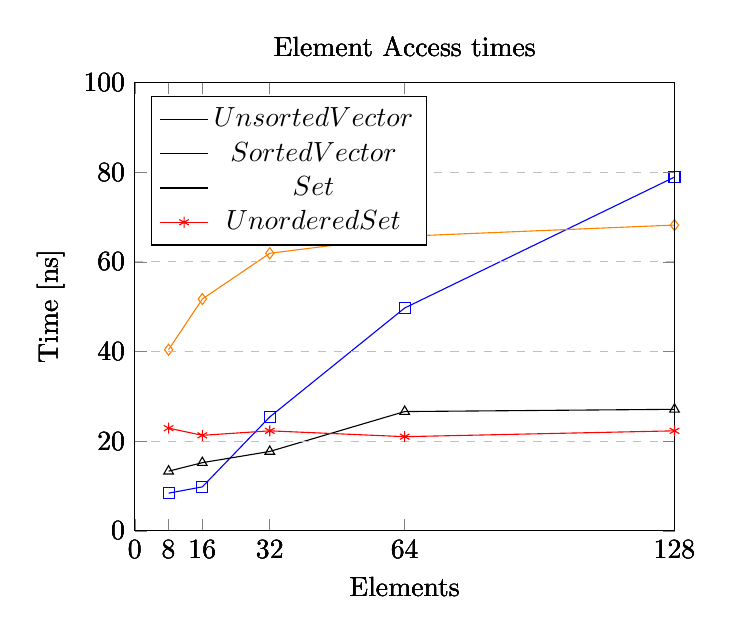
\begin{tikzpicture}
		\begin{axis}[
			title={Element Access times},
			xlabel={Elements},
			ylabel={Time [ns]},
			xmin=0, xmax=128,
			xtick={0,8,16,32,64,128},
			ymin=0, ymax=100,
			legend pos=north west,
			ymajorgrids=true,
			grid style=dashed
			]
			\addplot[
			color=blue,
			mark=square,
			]
			coordinates {			
				(8,8.4)(16,9.8)(32,25.4)(64,49.7)(128,78.9)
			};
			\label{Hplot}			
		\end{axis}
		
		\begin{axis}[
			title={Element Access times},
			xlabel={Elements},
			ylabel={Time [ns]},
			xmin=0, xmax=128,
			xtick={0,8,16,32,64,128},
			ymin=0, ymax=100,
			legend pos=north west,
			ymajorgrids=true,
			grid style=dashed
			]
			\addplot[
			color=black,
			mark=triangle,
			]
			coordinates {			
				(8,13.3)(16,15.2)(32,17.7)(64,26.6)(128,27.1)
			};
			\label{Bplot}			
		\end{axis}
		
		\begin{axis}[
			title={Element Access times},
			xlabel={Elements},
			ylabel={Time [ns]},
			xmin=0, xmax=128,
			xtick={0,8,16,32,64,128},
			ymin=0, ymax=100,
			legend pos=north west,
			ymajorgrids=true,
			grid style=dashed
			]
			\addplot[
			color=orange,
			mark=diamond,
			]
			coordinates {			
				(8,40.4)(16,51.7)(32,61.9)(64,65.7)(128,68.2)
			};
			\label{Cplot}			
		\end{axis}
		
		\begin{axis}[
			title={Element Access times},
			xlabel={Elements},
			ylabel={Time [ns]},
			xmin=0, xmax=128,
			xtick={0,8,16,32,64,128},
			ymin=0, ymax=100,
			legend pos=north west,
			ymajorgrids=true,
			grid style=dashed
			]
			\addlegendimage{/pgfplots/refstyle=Hplot}\addlegendentry{$Unsorted Vector$}
			\addlegendimage{/pgfplots/refstyle=Bplot}\addlegendentry{$Sorted Vector$}
			\addlegendimage{/pgfplots/refstyle=Cplot}\addlegendentry{$Set$}
			\addplot[
			color=red,
			mark=asterisk,
			]
			coordinates{
				(8,22.9)(16,21.3)(32,22.3)(64,21.0)(128,22.3)
			};
			\addlegendentry{$Unordered Set$}
		\end{axis}
	\end{tikzpicture}
	
	\lstlistoflistings
	\listoftables
	
\end{document}